\chapter{Trusted Platform Module}
The Trusted Platform Module is a system component used as a cryptographic co-processor. The TPM specification was defined and is currently maintained by Trusted Computing Group (TCG), formerly known as Trusted Computing Platform Alliance. The specification was also standardized by International Organization for Specification (ISO) and International Electrotechnical Commission (IEC) as ISO/IEC 11889.

This chapter introduces the basic concepts pertaining to TPMs, summarizes the history of their development, describes the TPM 2.0 specification, and reports on research also with regard to their various use cases. 

\section{Basic concepts}
This section provides an overview of basic concepts mentioned throughout this work.

\subsection{Trust, trusted, and trustworthy}\label{sec:trust-def}
The term "trust" has no uniformly formalized definition. Its interpretations vary even in the same field of study such as computer science and its subfields. The most relevant one for our needs is the TCGs' definition which states that trust is "the expectation that a device will behave in a particular manner for a specific purpose" \cite{tcg_arch_overview}. It is, however, important to note that this definition does not mention anything about the device being worthy of our trust. We only expect the specific behavior, and the device does not guarantee anything about its behavior. This means that a trusted device may fail us, whereas a trustworthy device is worthy of our trust and does not fail.

\subsection{Trusted Computing}
"Trusted computing refers to a computer system for which an entity has some level of assurance that the (part or all of) computer system behaves as expected" \cite{mitchell2005trusted}. In a sense, the definition of Trusted Computing presents a concept of trust in computing.

Schoen in \cite{schoen2003trusted} mentions these features of Trusted Computing:

\begin{itemize}

%\item \textbf{Endorsement Key} (EK) is a key stored permanently in TPM and is unique to each TPM. It is typically installed physically into the TPM during the manufacturing process. The EK consists of public and private key pair, where the private part never leaves the TPM. A certificate containing a public portion of EK and information about TPM can be signed by a certification authority to attest to the validity of EK and TPM itself. The EK is directly used only for the process of taking ownership of TPM and creating Attestation Identity Key  certificates \cite[p.~179-180]{Tomlinson2017}.

\item \textbf{Secure I/O} goal is to prevent spyware threats such as key loggers that record every keystroke or screen grabbers that adversaries may use to monitor user activities. Secure I/O provides a hardware "tunnel" between the user and the application so that no spying on the contents of their communication is possible.

\item \textbf{Memory Curtaining} pertains to a hardware memory isolation of processes so that they cannot modify each other's memory. According to the Trusted Computing design, even the operating system cannot access curtained memory. That means even if an attacker gains access to the system, they will not be able to tamper with curtained memory.

\item \textbf{Sealed Storage} is used for data protection. It enables the sealers to specify policies so that only designated parties can access the sealed data. This primitive uses two operations called Seal and Unseal. The Seal operation enables us to specify the access policy and seals the data. The Unseal operation checks if the unsealing entity adheres to the policy specified during sealing. If yes, then it unseals the data.

\item \textbf{Remote Attestation} is a process of proving some claim to the third party. The prover gathers the evidence to support their claim and presents it to the verifier, who, based on the evidence, decides if the prover is trustworthy for further interaction. In the Trusted Computing scenario, the claim to prove through remote attestation can be that the system runs only valid and unmodified software. 
\end{itemize}


\subsection{Roots of Trust}
Trust is a transitive relation; if component A trusts component B, and component B trusts component C, then component A must trust component C. If this relation is applied to a trusted platform, then one component trusts another, and so on. A chain of trust is created. This chain must end somewhere, that is at a so-called root of trust. However, if this root is not trustworthy and fails, it causes the whole chain to fail.

The trustworthiness of the roots of trust is essential. According to the TPM specification, the roots of trust "are system elements that must be trusted because misbehavior is not detectable" \cite[p.~23]{tcg_p1_architecture}, but their trustworthiness can be assured by knowing their implementation and providing the certification of this implementation.

There are three kinds of roots of trust required:
\begin{itemize}
    \item \textbf{Root of Trust for Measurement (RTM)} is trusted to reliably generate integrity measurements of software running on the platform. The measurements should ideally proceed from the boot of the platform. The entry point for the measurement is called Core Root of Trust for Measurement (CRTM), and it is generally found in the Bios boot block \cite[p.~185]{Tomlinson2017}. Generated integrity measurements are extended into PCR (see \myref{Section}{sec:pcr}) for the purpose of reporting.
    \item \textbf{Root of Trust for Storage (RTS)} is trusted to provide memory access control. The whole data it may protect is generally not stored in the Shielded Locations directly, but the TPM only guards a key to access the data stored externally. Although some memory locations in the TPM are not so sensitive to disclosure, such as a PCR and its current contents. 
    \item \textbf{Root of Trust for Reporting (RTR)} is trusted for reporting the current system state stored in RTS and attests to the authenticity of this information.
\end{itemize}


\section{History}
The development of the TPM specification spans multiple years and multiple versions of this specification. However, the most notable versions of the specification are TPM 1.1b, TPM 1.2, and the latest TPM 2.0. 

\subsection{TPM 1.1b}
The TPM 1.1b released in 2003 was the first broadly used TPM version. This specification already defined some essential functionality found in modern TPMs, such as:
\begin{itemize}
    \item \textbf{Cryptography} consisting of hashing, asymmetric key operations and random number generation.
    \item \textbf{Secure storage} to store secrets,
    \item \textbf{Endorsement Key and Attestation Identity Keys} for platform identity and attestation with cooperation of privacy CA,
    \item \textbf{Integrity collection and reporting} utilizing PCRs (see \myref{Section}{sec:pcr}).
\end{itemize}

\subsection{TPM 1.2}
The TPM 1.2 specification was in development from 2005 to 2009 when it was standardized as ISO/IEC 11889. Its final revision was in 2011. It resolved some problems of TPM 1.1b specification, notably a requirement for dictionary attack mitigation mechanisms was added \cite[p.~36-37]{tcg_1.2_design_princ}. This specification brought a lot of new functionality and features, for example:
\begin{itemize}
    \item \textbf{Direct Anonymous Attestation} \cite{daaSpec, daaDesignAndImple},
    \item \textbf{Locality} to differentiate commands between different sources,
    \item \textbf{Delegation}, where TPM owner can enable delegate access to specific owner-authorized commands,
    \item \textbf{Non-volatile storage} to store information,
    \item \textbf{Internal tick counter} used for timestamps,
    \item \textbf{Certified migration} of keys.
\end{itemize}
But there was also a lot of functionality that stayed the same as in TPM 1.1b. This is also related to the fact that the TPM 1.2 was required to keep the backward compatibility for TPM 1.1b \cite[p.~169]{tcg_1.2_design_princ}.

% TODO: PC specific Device interface was apparently defined in another specification
% https://trustedcomputinggroup.org/resource/pc-client-work-group-pc-client-specific-tpm-interface-specification-tis/

\subsection{TPM 2.0 reasoning}
One factor contributing to the need for yet another specification after TPM 1.2 was that in 2005, some substantial collision attacks were found against the SHA-1 hash function. Analysis regarding the use of SHA-1 in TPM revealed the attacks not being applicable~\cite{tcg_tpm1.12_sha-1_uses}. The SHA-1 hashing algorithm was used extensively in TPM 1.2. However, when its flaw was discovered, there was no way to replace it quickly. This problem fueled the idea that the new specification had to permit any hashing algorithm without making any changes to the specification. So-called digest agility. 

Another problem was the lack of a symmetric algorithm required in the TPM specification. The use of RSA for encryption of serialized data was impractical because RSA operations are slow. That's why it was decided that the following specification would adopt mandatory support for symmetric encryption, which is faster and more suitable for encryption of large byte streams. 


\section{TPM 2.0}\label{sec:tpm2}


The chance to overhaul the specification given to TPM 2.0 architects and developers, was turned into much more than support for digest agility and for symmetric cryptography algorithms. Support for algorithm agility was added which allows for various cryptographic primitives to be implemented with different algorithms. Authorization methods were unified and expanded, allowing for the building of complex authorization policies. TPM management was simplified in order for the TPM to be more useful to applications.

%First sentence is prob a nonsense
The main goal of the new specification was to provide a library describing features and commands available for implementation. This architecture allows designers to choose the required level of security, which may vary for different use cases. 

This section describes various types of TPMs, their basic features, and use cases.

\subsection{Types}
There is no single correct way how should TPM 2.0 be implemented. TPM specification does not dictate if a TPM should be implemented in hardware or software. Different usage scenarios may require a different type of TPM. The TPM specification only defines functionality to be adhered to by its implementations. 

According to \cite{tcg_tpm2_briefintro}, five types of a TPM are considered:

\begin{itemize}
    \item \textbf{Discrete TPM} is a hardware implementation of TPM specification. It is implemented as a standalone chip designed to be highly secure and tamper-proof. It can be used to protect even against very advanced attacks in security-critical infrastructures.
    \item \textbf{Integrated TPM} is still implemented in hardware, although as a part of a more complex chip, such as a CPU, which may have other responsibilities than security. They are not required to be tamper-resistant because such a requirement may immensely increase such chips' cost.
    \item \textbf{Firmware TPM} runs in the CPU's trusted execution environment (TEE), which protects and isolates the code and data along with providing confidentiality and integrity guarantees. Firmware TPM's security is very dependent on the TEE's security.
    \item \textbf{Virtual TPM} does not require a physical chip to be present. It entirely relies on the fact, that its users will be hypervisors, and the Virtual TPM itself will be isolated from the software running on the virtual machine to protect its code. 
    \item \textbf{Software TPM} is implemented as an emulator ideally used for testing and system prototyping purposes. It does not run inside of an isolated environment and may be prone to tampering.
\end{itemize}

\subsection{Features}

\subsubsection{Platform Configuration Registers}\label{sec:pcr}
Platform Configuration Registers (PCRs) are dynamic memory locations inside a TPM used to store integrity metrics of software and its configuration. These locations can only be updated using \texttt{extend} operation and also read for reporting or attestation. The \texttt{extend} operation makes use of the cryptographic hash function to combine the digest stored in the PCR and the new data. Cryptographic hash function map data of arbitrary size to the output of a fixed size. Such outputs are conventionally called hashes, message digests, or digests. These functions have one-way property: when given a message digest, it is difficult  to compute the message itself. The extend operation works in the following way:
\begin{align*}
    d_{n+1} = h(d_{n}\ ||\ data)
\end{align*}
\begin{itemize}
    \item $||$ is a concatenation of data in binary form
    \item $ d_{n} $ is a digest stored in PCR before \texttt{extend} operation
    \item $ d_{n+1} $ is a digest stored in PCR after \texttt{extend} operation
    \item $ data $ is binary data to extend by
    \item $ h $ is a cryptographic hash function
\end{itemize}

We can always recompute the final value if we possess the knowledge of members previously used in the chain and detect potential alterations.




\subsection{Architecture}
Although there is no prescribed form of TPM in terms of hardware or software, the specification requires its implementations to possess several functional components for its operation~\cite{tcg_p1_architecture}. Selection of important building blocks of TPM is shown in \myref{Figure}{fig:tpm-arch-scheme}.

\begin{figure}[H]
    \centering
    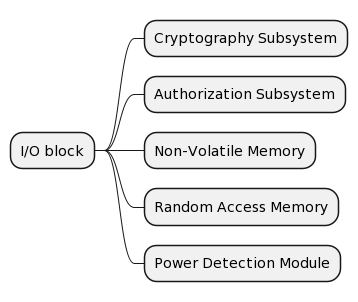
\includegraphics[width=\textwidth-6cm]{img/tpm-arch-diagram.png}
    \caption{Important blocks of TPM architecture}
    \label{fig:tpm-arch-scheme}
\end{figure}

\begin{itemize}

\item \textbf{I/O Buffer} is a location used for communication between the host platform and TPM. A precise description of interfaces used for communication is left up to designers of such interfaces.

\item \textbf{Cryptography Subsystem} which provides implementations of various cryptographic primitives, most of which may be used by other modules. These primitives generally consist of: 
\begin{itemize}
    \item Hash functions which may be used by external software, different TPM operations such as PCR extend, or other cryptographic primitives. 
    \item Symmetric cryptography provides means of symmetric encryption and decryption along with various block cipher modes of operation.
    \item Asymmetric cryptography is used for signatures, signature verification, and shared secret establishment. The only supported algorithms are RSA and ECC.
    \item Message Authentication Codes use either the beforementioned hashing capabilities (HMAC) or symmetric ones (SMAC).
    \item Random Number Generator is used as a source of randomness in TPM. The randomness is necessary for the generation of nonces and keys and for signatures. 
    \item Key Generation uses RNG value either directly as a secret key or as a seed to derive from applying some approved key derivation function.
\end{itemize}

\item \textbf{Authorization Subsystem} which tests that each executed command has required authorization to access Shielded Locations. 

\todo{Explain Shielded Locations}
\item \textbf{Non-Volatile Memory} provides persistent storage space for allocation and contains Shielded Locations.

\item \textbf{Random Access Memory} provides storage space that is not required to be persistent. It also contains Shielded Locations, most notably PCRs of which accumulative property is used to process logs of system state which may be subsequently validated. This is particularly useful when we want to measure the boot sequence of the system so that no malicious changes may be applied to it.

\item \textbf{Power Detection Module} handles TPM power states according to platform power state changes.
\end{itemize}

\section{Use cases}
In this section, the use cases for TPM will be discussed in order from more traditional ones to more specific and state-of-the-art ones.

\subsection{Measured boot}

\subsection{Storage Encryption}

\subsection{Digital Rights Management}

\subsection{State-of-the-art cryptography using TPM commands}
The TPMs contain only specific widely used cryptographic primitives. These primitives can be used either independently by calling the corresponding commands from the TPM specification or as building blocks of more complex cryptographic protocols and schemes. 

The TPM 2.0 provides one signature primitive, which enables the implementation of signature schemes and cryptographic protocols using this primitive \cite{chen2013flexible}. This primitive is implemented in TPM 2.0 using five commands:
\begin{itemize}
    \item \textbf{TPM2\_Create} or \textbf{TPM2\_CreatePrimary} which are used for the generation of asymmetric key pairs. The difference between the two is that the latter one's key generation uses a special secret key stored in the TPM as a seed.
    \item \textbf{TPM2\_Load} which loads the key into the TPM. For the TPM to work with the key, the TPM must load it because the previously created key may not be stored inside the TPM.
    \item \textbf{TPM2\_ActivateCredential} which is used to certify the created key. The public portion of the generated key and public portion of TPM's endorsement key is sent by the platform associated with TPM to the Certification Authority, which checks the validity of TPM's endorsement key and creates a certificate for the generated key and a symmetric key. Then it sends both back to the platform.
    \item \textbf{TPM2\_Commit} is the first but optional part of the signing process defined in \cite{chen2013flexible}. The TPM generates commitment and returns associated values and a reference to the commitment value. The reference to the commitment is just a simple identifier based on which the TPM can recompute the commitment value. Commitments are fundamentally used in most cryptographic schemes and protocols. For more information about commitments in cryptographic schemes and protocols, see~\cite{damgaard1998commitment}. 
    \item \textbf{TPM2\_Sign} which is used to sign a given message. Generally, only the hash of the given message is signed. If a TPM2\_Commit command was called before and the signature algorithm uses commitments, then the commitment value is retrieved using the reference provided by the TPM2\_Commit command.
\end{itemize}
Chen and Li~\cite{chen2013flexible} also discuss the possible applications of this signature primitive for implementing protocols and schemes such as Direct Anonymous Attestation~\cite{daaSpec}, U-Prove~\cite{uproveSpec}, or more conventional signature schemes such as Schnorr signatures~\cite{schnorrSpec}. 
% Though the ECC-DAA is adopted by TPM specification, it would be probably good to mention it.

Several papers proposed various schemes using the beforementioned signature primitive in TPM 2.0. Generally most of them propose attestation schemes. 

Kumar et. al~\cite{kumar2018direct} proposes DAA scheme based on ECC and addresses the problem of effective revocation in subscription systems. Subscription systems allow its subscribers to access resources. Example of that may be streaming platform which provides service of viewing movies where the subscriber needs to pay a subscription fee to be able to access this service. In such systems it may be important for the provider to be able to revoke the access to services provided by these systems. Kumar et. al consider DAA as an ideal protocol for realization of these subscription systems. Their scheme is called LASER which stands for Lightweight Anonymous Subscription with Efficient Revocation and implement this scheme using TPM in compliance to TPM 2.0 specification. They also provide a reference implementation of this scheme, which is publicly available on GitHub\footnote{\url{https://github.com/luthern/laser}}. 

Another DAA scheme was proposed by Wesemeyer et. al \cite{wesemeyerDAA} which extends ECC-DAA defined by Chen and Li \cite{chen2013flexible}. They provide thorough formal verification using security verification tool called Tamarin prover \cite{meier2013tamarin} and most importantly provide implementation details of the scheme along with it's reference implementation.

Wagner, Birnstill and Beyerer \cite{wagnerRemoteAttProtocol} propose remote attestation protocol based on TPM 2.0 specification which provides attestation, re-attestation, and establishment of shared key. This protocol may be used for establishment of encrypted channel between trusted platforms. Their protocol is designed to be immune to replay, insider attacks and two specific relay attacks. They also performed a formal verification of their
protocol using Tamarin prover \cite{meier2013tamarin}, though the authors do not elaborate much on the process of formal verification they performed.

Hedabou and Abdulsalam \cite{hedabou2020efficient} propose a multi-signature scheme on TPM based on BLS digital signature. The specific property of this multi-signature scheme is that it is non-interactive, meaning that the multi-signature does not require interaction between the signing parties. Their proposed scheme shows high signing efficiency and compared it to signature schemes \cite{chen2013flexible} and \cite{schnorrSpec}. An analysis showing respectable latency and computational time with up to thousand of participating signers shows that their scheme may be usable for cryptocurrency applications.





\section{Research}

\subsection{Security analysis}

\subsection{Performance analysis}

%\subsection{tpm2-algtest}
%The \texttt{tpm2-algtest}\footnote{https://github.com/crocs-muni/tpm2-algtest} is a tool for automatic gathering of information about the TPM2 devices \cite{Struk2019thesis}. The tool uses libraries implementing Trusted Computing Group's TPM2 Software Stack\footnote{https://github.com/tpm2-software/tpm2-tss} which allows for simplification of development when programming applications supposed to interact with the TPM. The tool tests for support of specific commands and supporting routines, values of structures defined in the TPM 2.0 specification \cite{tcg_p3_commands, tcg_p4_supproutines, tcg_p2_structures}. Supported cryptographic algorithms are also subject to performance analysis where the time to execute such an algorithm is repeatedly measured and recorded. Additionally, the tool uses the TPM to generate key pairs for RSA and ECC-based algorithms so that they can be further analyzed by various means.
